%
% Copyright 2018 Joel Feldman, Andrew Rechnitzer and Elyse Yeager.
% This work is licensed under a Creative Commons Attribution-NonCommercial-ShareAlike 4.0 International License.
% https://creativecommons.org/licenses/by-nc-sa/4.0/
%
\questionheader{ex:s1.12}
%{rmk:singularities} - using with singularities
%%%%%%%%%%%%%%%%%%
\subsection*{\Conceptual}
%%%%%%%%%%%%%%%%%%
\begin{Mquestion}
For which values of $b$ is the integral
$\displaystyle\int_0^b \frac{1}{x^2-1}~\dee{x}$ improper?
\end{Mquestion}
\begin{hint}
There are two kinds of impropreity in an integral: an infinite discontinuity in the integrand, and an infinite limit of integration.
\end{hint}
\begin{answer}
Any real number in $[1,\infty)$ or $(-\infty,-1]$, and $b = \pm \infty$.
\end{answer}
\begin{solution}
If $ = \pm \infty$, then our integral is improper because one limit is not a real number.

Furthermore, our integral will be improper if its domain of integration contains either of its infinite discontinuities, $x=1$ and $x=-1$. Since one limit of integration is 0, the integral is improper if $b \geq 1$ or if $b \leq -1$.

Below, we've graphed $\frac{1}{x^2-1}$ to make it clearer why values of $b$ in $(-1,1)$ are the only values that \emph{don't} result in an improper integral when the other limit of integration is $a=0$.

\begin{center}
\begin{tikzpicture}
\YEaaxis{3.3}{3.3}{3}{2.5}
\draw[thick, blue] plot[domain=-.8:.8](\x,{1/(\x*\x-1)});
\draw[thick, blue] plot[domain=-3:-1.2](\x,{1/(\x*\x-1)});
\draw[thick, blue] plot[domain=1.2:3](\x,{1/(\x*\x-1)}) node[above]{$y = \frac{1}{x^2-1}$};
\draw[ blue, dashed] (-1,-2.8)-- (-1,-.7) (-1,.3)--(-1,2.3) (1,-2.8)--(1,-.7) (1,.3)--(1,2.3);
\YExcoord{-1}{-1}
\YExcoord{1}{1}
\end{tikzpicture}
\end{center}
\end{solution}
%%%%%%%%%%%%%%%%%%%
\begin{Mquestion}
For which values of $b$ is the integral
$\displaystyle\int_0^b \frac{1}{x^2+1}~\dee{x}$ improper?
\end{Mquestion}
\begin{hint}
The integrand is continuous for all $x$.
\end{hint}
\begin{answer}
$b = \pm\infty$
\end{answer}
\begin{solution}
Since the integrand is continuous for all real $x$, the only kind of impropriety available to us is to set $b = \pm\infty$.
\end{solution}
%%%%%%%%%%%%%%%%%%%

\begin{Mquestion}
Below are the graphs $y=f(x)$ and $y=g(x)$. Suppose $\displaystyle\int_0^\infty f(x)~\dee{x}$ converges, and $\displaystyle\int_0^\infty g(x)~\dee{x}$ diverges. Assuming the graphs continue on as shown as $x \to \infty$, which graph is $f(x)$, and which is $g(x)$?
\begin{center}
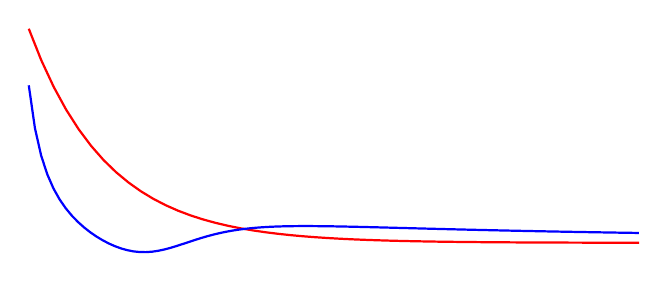
\begin{tikzpicture}
\YEaaxis{1}{7}{1}{3}
\draw[thick, red] plot[domain=-1:6.75, samples=50](\x,{1/exp(\x)});
\draw[thick, blue] plot[domain=-1:6.75, samples=100](\x,{\x*(\x-1)/(\x^3+2)});
\end{tikzpicture}
\end{center}

\end{Mquestion}
\begin{hint}
What matters is which function is bigger for large values of $x$, not  near the origin.
\end{hint}
\begin{answer}
The red function is $f(x)$, and the blue function is $g(x)$.
\end{answer}
\begin{solution}
For large values of $x$, $|\text{red function}|\leq \text{(blue function)}$ and $0 \leq \text{(blue function)}$. If the blue function's integral converged, then the red function's integral would as well (by the comparison test, Theorem~\eref{CLP101}{thm:IMPcomparison} in the CLP--II text). Since one integral converges and the other diverges, the blue function is $g(x)$ and the red function is $f(x)$.
\end{solution}
%%%%%%%%%%%%%%%%%%%
\begin{question}[2015A]
Decide whether the following statement is true or false.
If false, provide a counterexample. If true, provide a brief justification.
(Assume that $f(x)$ and $g(x)$ are continuous functions.)

\begin{enumerate}[(a)]
\item []
If $\displaystyle\int_{1}^{\infty} f(x) \,\dee{x}$ converges and $g(x)\ge f(x)\ge 0$ for all $x$, then $\displaystyle\int_{1}^{\infty} g(x) \,\dee{x}$ converges.
\end{enumerate}
\end{question}

\begin{hint}
Read both the question and Theorem \eref{CLP101}{thm:IMPcomparison} in the
%\href{http://www.math.ubc.ca/%7Efeldman/m101/clp/clp_notes_101.pdf}{CLP--II text}.
CLP--II text \emph{very} carefully.
\end{hint}

\begin{answer}
False. For example, the functions $f(x)=e^{-x}$ and $g(x)=1$ provide a counterexample.


\end{answer}

\begin{solution}
False. The inequality goes the ``wrong way" for Theorem \eref{CLP101}{thm:IMPcomparison}
 in the CLP--II text: the area under the curve $f(x)$ is finite, but the area under $g(x)$ could be much larger, even infinitely larger.

 For example, if $f(x)=e^{-x}$ and $g(x)=1$,
then $0 \leq f(x) \leq g(x)$ and $\displaystyle\int_{1}^{\infty} f(x) \,\dee{x}$ converges, but
$\displaystyle\int_{1}^{\infty} g(x) \,\dee{x}$ diverges.
\end{solution}
%%%%%%%%%%%%%%%%%%%

\begin{question}
Let $f(x) = e^{-x}$ and $g(x)=\dfrac{1}{x+1}$. Note $\int_{0}^\infty f(x)~\dee{x}$ converges while
$\int_{0}^\infty g(x)~\dee{x}$ diverges.

For each of the functions $h(x)$ described below, decide whether $\int_{0\vphantom{\frac12}}^\infty h(x)~\dee{x}$ converges or diverges, or whether there isn't enough information to decide. Justify your decision.

\begin{enumerate}[(a)]
\item $h(x)$, continuous and defined for all $x \ge0$, $h(x) \leq f(x)$.
\item $h(x)$, continuous and defined for all $x\ge 0$, $f(x) \leq h(x) \leq g(x)$.
\item $h(x)$, continuous and defined for all $x\ge 0$, $-2f(x) \leq h(x) \leq f(x)$.
\end{enumerate}
\end{question}
\begin{hint}
(a) What if $h(x)$ is negative? What if it's not?\\
(b) What if $h(x)$ is very close to $f(x)$ or $g(x)$, rather than right in the middle?\\
(c) Note $|h(x)| \leq 2f(x)$.
\end{hint}
\begin{answer}
\begin{enumerate}[(a)]
\item Not enough information to decide. For example, consider $h(x) = 0$ versus $h(x) = -1$.
\item Not enough information to decide. For example, consider $h(x)= f(x)$ versus $h(x) = g(x)$.
\item $\displaystyle\int_{0\vphantom{\frac12}}^{\infty}h(x)~\dee{x}$ converges by the comparison test, since $|h(x)| \leq 2f(x)$ and $\displaystyle\int_0^\infty 2f(x)~\dee{x}$ converges.
\end{enumerate}
\end{answer}
\begin{solution}
\begin{enumerate}[(a)]
\item Not enough information to decide. For example, consider $h(x) = 0$ versus $h(x) = -1$. In both cases, $h(x) \leq f(x)$. However, $\displaystyle\int_0^\infty 0~\dee{x}$ converges to 0, while $\displaystyle\int_0^\infty -1~\dee{x}$ diverges.

Note: if we had also specified $0 \leq h(x)$, then we would be able to conclude that $ \int_0^\infty h(x)~\dee{x}$ converges by the comparison test.

\item Not enough information to decide. For example, consider $h(x)= f(x)$ versus $h(x) = g(x)$. In both cases, $f(x) \leq h(x) \leq g(x)$.

\item $\displaystyle\int_{0\vphantom{\frac12}}^{\infty}h(x)~\dee{x}$ converges.
\begin{itemize}
\item From the given information, $|h(x)| \leq 2f(x)$.
\item We claim $\displaystyle\int_{0\vphantom{\frac12}}^{\infty} 2f(x)~\dee{x} $ converges.
\begin{itemize}
\item We can see this by writing $\displaystyle\int_{0\vphantom{\frac12}}^{\infty} 2f(x)~\dee{x}= 2\int_0^{\infty} f(x)~\dee{x} $  and noting that the second integral converges. \item Alternately, we can use  the limiting comparison test, Theorem~\eref{CLP101}{thm:IMPcomparisonLim}
 in the CLP--II text. Since $f(x) \geq 0$,  $\displaystyle\int_0^\infty f(x)~\dee{x}$ converges, and $\lim\limits_{x \to \infty}\dfrac{2f(x)}{f(x)}=2$ (the limit exists), we conclude $\displaystyle\int_0^\infty 2f(x)~\dee{x}$ converges.
\end{itemize}
\item So, comparing $h(x)$ to $2f(x)$, by the comparison test (Theorem~\eref{CLP101}{thm:IMPcomparison} in the CLP--II text)
$\displaystyle\int_0^{\vphantom{\frac12}\infty}h(x)~\dee{x}$ converges.
\end{itemize}
\end{enumerate}

\end{solution}



%%%%%%%%%%%%%%%%%%
\subsection*{\Procedural}
%%%%%%%%%%%%%%%%%%

\begin{Mquestion}[M105 2015A]
Evaluate the integral
$\displaystyle\int_0^1\frac{x^4}{x^5-1}\,\dee{x}$ or state that
it diverges.
\end{Mquestion}

\begin{hint}
First: is the integrand unbounded, and if so, where?

Second: when evaluating integrals, always check to see if you can use a simple
substitution before trying a complicated procedure like partial fractions.
\end{hint}

\begin{answer}
The integral diverges.
\end{answer}

\begin{solution}
The denominator is zero when $x=1$, but the numerator is not, so the integrand has a
singularity (infinite discontinuity) at $x=1$. Let's replace the limit $x=1$ with a variable that creeps toward 1.
\begin{equation*}
\int_0^1\frac{x^4}{x^5-1}\,\dee{x}
=\lim_{t\rightarrow 1^-}\int_0^t\frac{x^4}{x^5-1}\,\dee{x}
\end{equation*}
To evaluate this integral we use the substitution
$u=x^5$, $\dee{u}=5x^4\dee{x}$. When $x=0$ we have $u=0$, and when $x=t$
we have $u=t^5$, so
\begin{align*}
\int_0^1\frac{x^4}{x^5-1}\,\dee{x}&=\lim_{t \to 1^-}\int_{0}^{t}\frac{x^4}{x^5-1}\,\dee{x}
=\lim_{t \to 1^-}\int_{u=0}^{u=t^5}\frac{1}{5(u-1)}\,\dee{u}\\
&=\lim_{t \to 1^-}\left( \left[\frac{1}{5}\log|u-1|\right]_0^{t^5}\right)
=\lim_{t \to 1^-}\frac{1}{5}\log|t^5-1|=-\infty
\end{align*}
The limit diverges, so the integral diverges as well.
\end{solution}
%%%%%%%%%%%%%%%%%%%




\begin{question}[2016Q4]
Determine whether the integral
$\displaystyle\int_{-2}^2\frac{1}{(x+1)^{4/3}}\,\dee{x}$ is convergent
or divergent. If it is convergent, find its value.
\end{question}

\begin{hint}
Is the integrand bounded?
\end{hint}

\begin{answer}
The integral diverges.
\end{answer}

\begin{solution}
The denominator of the integrand is zero when $x=-1$, but the numerator is not. So, the integrand has a singularity (infinite discontinuity) at $x=-1$. This is the only ``source of impropriety" in this integral, so we only need to make one break in the domain of integration.
\begin{equation*}
\int_{-2}^2\frac{1}{(x+1)^{4/3}}\,\dee{x}
=\lim_{t\rightarrow -1^-}\int_{-2}^t \frac{1}{(x+1)^{4/3}}\,\dee{x}
  +\lim_{t\rightarrow -1^+}\int_t^2 \frac{1}{(x+1)^{4/3}}\,\dee{x}
\end{equation*}
Let's start by considering the left limit.
\begin{align*}
\lim_{t \to -1^-}\int_{-2}^t \frac{1}{(x+1)^{4/3}}\,\dee{x}
&=\lim_{t \to -1^-}\left(\left[-\frac{3}{(x+1)^{1/3}}\right|_{-2}^t\right)\\
&=\lim_{t \to -1^-}\left(-\frac{3}{(t+1)^{1/3}}+\frac{3}{(-1)^{1/3}}\right)=\infty
\end{align*}
Since this limit diverges, the integral diverges. (A similar argument shows
that the second integral diverges. Either one of them diverging is enough to conclude that the
original integral diverges.)
\end{solution}
%%%%%%%%%%%%%%%%%%%


\begin{question}[1997D]
 Does the improper integral
$\displaystyle\int_1^\infty\frac{1}{\sqrt{4x^2-x}}\,\dee{x}$ converge? Justify your
answer.
\end{question}

\begin{hint}
See Example \eref{CLP101}{eg:IMPp10} in the
%\href{http://www.math.ubc.ca/%7Efeldman/m101/clp/clp_notes_101.pdf#section1.6}{CLP--II text}.
%\href{http://www.math.ubc.ca/%7Efeldman/m101/clp/clp_notes_101.pdf}{CLP--II text}.
CLP--II text. Rather than antidifferentiating, you can find a nice comparison.
\end{hint}

\begin{answer}
The integral does not converge.
\end{answer}

\begin{solution}
First, let's identify all ``sources of impropriety." The integrand has a singularity when $4x^2-x=0$, that is, when $x(4x-1)=0$, so at $x=0$ and $x=\frac{1}{4}$. Neither of these are in our domain of integration, so the only ``source of impropriety" is the unbounded domain of integration.

We could antidifferentiate this function (it looks like a nice candidate for a trig substitution), but is seems easier to use a comparison. For large values of $x$, the term $x^2$ will be much larger than $x$, so we might guess that our integral behaves similarly to $\int_1^\infty \frac{1}{\sqrt{4x^2}}~\dee{x}=\int_1^\infty \frac{1}{2x}~\dee{x}$.


For all $x\ge 1$, $\sqrt{4x^2-x}\le\sqrt{4x^2}=2x$. So, $\frac{1}{\sqrt{4x^2-x}} \geq \frac{1}{2x}$. Note $\int_1^\infty \frac{1}{2x}~\dee{x}$ diverges:
\begin{align*}\lim_{t\rightarrow\infty}\int_1^t\frac{1}{2x}\,\dee{x}
=\lim_{t\rightarrow\infty}\left(\frac{1}{2} \big[\log x\big]_1^t\right)
=\lim_{t\rightarrow\infty}\frac{1}{2} \log t
=\infty
\end{align*}
So:
\begin{itemize}
\item $\frac{1}{2x}$ and $\frac{1}{\sqrt{4x^2-x}}$ are defined and continuous for all $x \geq 1$,
\item $\frac{1}{2x} \geq 0$ for all $x \geq 1$,
\item $\frac{1}{\sqrt{4x^2-x}} \ge\frac{1}{\sqrt{4x^2}} = \frac{1}{2x} $ for all $x \ge 1$, and
\item $\int_1^\infty \frac{1}{2x}~\dee{x}$ diverges.
\end{itemize}
By the comparison test, Theorem~\eref{CLP101}{thm:IMPcomparison} in the CLP--II text, the integral does not converge.
\end{solution}
%%%%%%%%%%%%%%%%%%%

\begin{Mquestion}[2001A]
Does the integral $\displaystyle\int_0^\infty\frac{\dee{x}}{x^2+\sqrt{x}}$
converge or diverge? Justify your claim.
\end{Mquestion}

\begin{hint}
Which of the two terms in the denominator is more important when $x\approx
0$? Which one is more important when $x$ is very large?
\end{hint}

\begin{answer}
The integral converges.
\end{answer}

\begin{solution}
The integrand is positive everywhere. So, either the integral
converges to some finite number, or it is infinite. We want to generate a guess as to which it is.

When $x$ is small, $\sqrt{x}>x^2$, so we might guess that our integral behaves like the integral of $\frac{1}{\sqrt{x}}$ when $x$ is near to 0. On the other hand, when $x$ is large, $\sqrt{x}<x^2$, so we might guess that our integral behaves like the integral of $\frac{1}{x^2}$ as $x$ goes to infinity.  This is the hunch that drives the following work:
\begin{alignat*}{3}
0\le\frac{1}{x^2+\sqrt{x}}
&\le \frac{1}{\sqrt{x}}\quad
&&\text{and the integral }\int_0^1\frac{\dee{x}}{\sqrt{x}}\text{ converges
by Example \eref{CLP101}{eg:IMPp2} in the CLP--II text, and} \\
0\le\frac{1}{x^2+\sqrt{x}}
&\le \frac{1}{x^2}
&&\text{and the integral }\int_1^\infty\frac{\dee{x}}{x^2}\text{ converges
by Example \eref{CLP101}{eg:IMPp1} in the CLP--II text}
\end{alignat*}
Note $\frac{\dee{x}}{x^2+\sqrt{x}}$ is defined and continuous everywhere, $\frac{1}{\sqrt{x}}$ is defined and continuous for $x>0$, and $\frac{1}{x^2}$ is defined and continuous for $x \ge 1$.
So, the integral converges by the comparison test, Theorem~\eref{CLP101}{thm:IMPcomparison} in the CLP--II text, together with Remark~\eref{CLP101}{rmk:singularities}.

\end{solution}
%%%%%%%%%%%%%%%%%%%
\begin{question}\label{prob_s1.11_cosine}
Does the integral $\displaystyle\int_{-\infty}^\infty \cos x~\dee{x}$ converge or diverge?
 If it converges, evaluate it.
\end{question}
\begin{hint}
Remember to break the integral into two pieces.
\end{hint}
\begin{answer}
The integral diverges.
\end{answer}
\begin{solution}
There are two ``sources of impropriety:" the two (infinite) limits of integration. So, we break our integral into two pieces.
\begin{align*}
\int_{-\infty}^\infty \cos x~\dee{x}&=\int_{-\infty}^0 \cos x~\dee{x}+\int_{0}^\infty \cos x~\dee{x}\\
&=\lim_{a \to \infty }\left[\int_{-a}^0 \cos x~\dee{x}\right]+
\lim_{b \to \infty }\left[\int_{0}^b \cos x~\dee{x}\right]
\intertext{These are easy enough to antdifferentiate.}
&=\lim_{a \to \infty }\left[\sin 0 - \sin(- a)
\right]+
\lim_{b \to \infty }\left[\sin b - \sin 0
\right]\\
&=\text{DNE}
\end{align*}
Since the limits don't exist, the integral diverges. (It happens that both limits don't exist; even if only one failed to exist, the integral would still diverge.)
\end{solution}
%%%%%%%%%%%%%%%%%%%
\begin{Mquestion}\label{prob_s1.11_sine}
Does the integral $\displaystyle\int_{-\infty}^\infty \sin x~\dee{x}$ converge or diverge?
 If it converges, evaluate it.
\end{Mquestion}
\begin{hint}
Remember to break the integral into two pieces.
\end{hint}
\begin{answer}
The integral diverges.
\end{answer}
\begin{solution}
There are two ``sources of impropriety:" the two bounds. So, we break our integral into two pieces.
\begin{align*}
\int_{-\infty}^\infty \sin x~\dee{x}&=\int_{-\infty}^0 \sin x~\dee{x}+\int_{0}^\infty \sin x~\dee{x}\\
&=\lim_{a \to \infty }\left[\int_{-a}^0 \sin x~\dee{x}\right]+
\lim_{b \to \infty }\left[\int_{0}^b \sin x~\dee{x}\right]\\
&=\lim_{a \to \infty }\left[-\cos 0 + \cos(- a)
\right]+
\lim_{b \to \infty }\left[-\cos b + \cos 0
\right]\\
&=\text{DNE}
\end{align*}
Since the limits don't exist, the integral diverges. (It happens that both limits don't exist; even if only one failed to exist, the integral would diverge.)

Remark: it's very tempting to think that this integral should converge, because as an odd function the area to the right of the $x$-axis ``cancels out" the area to the left when the limits of integration are symmetric. One justification for not using this intuition is given in Example~\eref{CLP101}{eg:IMPp4} in the CLP--II text. Here's another:
In Question~\ref{prob_s1.11_cosine} we saw that $\int_{-\infty}^\infty \cos x~\dee{x}$ diverges. Since $\sin x = \cos (x-\pi/2)$, the area bounded by sine and the area bounded by cosine over an infinite region seem to be the same--only shifted by $\pi/2$. So if $\int_{-\infty}^\infty \sin x~\dee{x}=0$, then we ought to also have $\int_{-\infty}^\infty \cos x~\dee{x}=0$, but we saw in Question~\ref{prob_s1.11_cosine} this is not the case.

\begin{center}
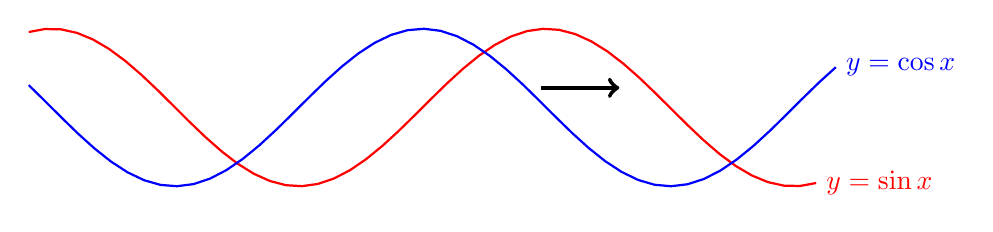
\begin{tikzpicture}
\YEaxis{5}{2}
\draw[thick, red] plot[domain = -5:5, samples=50](\x,{sin(\x r)}) node[right]{$y=\sin x$};
\draw[thick, blue] plot[domain = -5:5.25, samples=50](\x,{cos(\x r)}) node[right]{$y=\cos x$};
\draw[ultra thick, ->] (1.5,.25)--(2.5,.25);
\end{tikzpicture}
\end{center}
\end{solution}

%%%%%%%%%%%%%%%%%%%
\begin{question}
Evaluate $\displaystyle\int_{10}^\infty \frac{x^4-5x^3+2x-7}{x^5+3x+8} ~\dee{x}$, or state that it diverges.
\end{question}
\begin{hint}
The easiest test in this case is  limiting comparison, Theorem~\eref{CLP101}{thm:IMPcomparisonLim} in the CLP--II text.
\end{hint}
\begin{answer}
The integral diverges.
\end{answer}
\begin{solution}
First, we check that the integrand has no singularities. The denominator is always positive when $x \ge 10$, so our only ``source of impropriety" is the infinite limit of integration.

We further note that, for large values of $x$, the integrand resembles $\dfrac{x^4}{x^5} = \dfrac{1}{x\vphantom{\frac12}}$. So, we have a two-part hunch: that the integral diverges, and that we can show it diverges by comparing it to $\displaystyle\int_{10}^\infty \frac{1}{x}~\dee{x}$.

In order to use the comparison test, we'd need to show that $\displaystyle\frac{x^4-5x^3+2x-7}{x^5+3x+8}  \geq \frac{1}{\vphantom{\frac12}x}$. If this is true, it will be difficult to prove--and it's not at all clear that it's true. So, we will use the limiting comparison test instead, Theorem~\eref{CLP101}{thm:IMPcomparisonLim} in the CLP--II text, with $g(x)= \dfrac{1}{x}$,
$f(x)=\dfrac{x^4-5x^3+2x-7}{x^5+3x+8} $, and $a=10$.

\begin{itemize}
\item Both $f(x)$ and $g(x)$ are defined and continuous for all $x >0$, so in particular they are defined and continuous for $x \geq 10$.
\item $g(x) \geq 0$ for all $x \geq 10$
\item $\displaystyle\int_{10}^\infty g(x)~\dee{x}$ diverges.
\item Using  l'H\^opital's rule (5 times!), or simply dividing both the numerator
           and denominator by $x^5$ (the common leading term), tells us:
\begin{align*}
\lim_{x \to \infty} \frac{f(x)}{g(x)}&=
\lim_{x \to \infty} \frac{\frac{x^4-5x^3+2x-7}{x^5+3x+8} }{ \frac{1}{x}}=
\lim_{x \to \infty} x\cdot\frac{x^4-5x^3+2x-7}{x^5+3x+8} \\
&=\lim_{x \to \infty} \frac{x^5-5x^4+2x^2-7x}{x^5+3x+8} =1
\end{align*}
That is, the limit exists and is nonzero.
\end{itemize}
By the limiting comparison test, we conclude $\displaystyle\int_{10}^\infty f(x)~\dee{x}$ diverges.
\end{solution}
%%%%%%%%%%%%%%%%%%%
\begin{Mquestion}
Evaluate $\displaystyle\int_0^{10} \frac{x-1}{x^2-11x+10} ~\dee{x}$, or state that it diverges.
\end{Mquestion}
\begin{hint}
Not all discontinuities cause an integral to be improper--only infinite discontinuities.
\end{hint}
\begin{answer}
The integral diverges.
\end{answer}
\begin{solution}
Our domain of integration is finite, so the only potential ``sources of impropriety" are infinite discontinuities in the integrand. To find these, we factor.
\begin{align*}
\int_0^{10} \frac{x-1}{x^2-11x+10} ~\dee{x}&=
\int_0^{10} \frac{x-1}{(x-1)(x-10)} ~\dee{x}
\intertext{A removable discontinuity doesn't affect the integral.}
&=\int_0^{10} \frac{1}{x-10} ~\dee{x}\\
\intertext{Use the substitution $u=x-10$, $\dee{u}=\dee{x}$. When $x=0$, $u=-10$, and when $x=10$, $u=0$.}
&=\int_{-10}^0 \frac{1}{u}~\dee{u}
\end{align*}
This is a $p$-integral with $p=1$. From Example~\eref{CLP101}{eg:IMPp2} and Theorem~\eref{CLP101}{thm:IMPfiniteSHift} in the CLP--II text, we know it diverges.
\end{solution}
%%%%%%%%%%%%%%%%%%%



\begin{question}[M121 2012A]
Determine (with justification!) which of the following applies to the integral
$\displaystyle\int_{-\infty}^{+\infty}\frac{x}{x^2+1}\dee{x}$:
\begin{enumerate}[(i)]
\item $\displaystyle\int_{-\infty}^{+\infty}\frac{x}{x^2+1}\dee{x}$ diverges
\item $\displaystyle\int_{-\infty}^{+\infty}\frac{x}{x^2+1}\dee{x}$ converges but
$\displaystyle\int_{-\infty}^{+\infty}\left|\frac{x}{x^2+1}\right|\dee{x}$ diverges
\item $\displaystyle\int_{-\infty}^{+\infty}\frac{x}{x^2+1}\dee{x}$
 converges, as does $\displaystyle\int_{-\infty}^{+\infty}\left|\frac{x}{x^2+1}\right|\dee{x}$
\end{enumerate}
Remark: these options, respectively, are that the integral diverges, converges conditionally, and converges absolutely. You'll see this terminology used for series in
Section~\eref{CLP101}{sec:abs conv} of the CLP--II text.
\end{question}

\begin{hint}
Which of the two terms in the denominator is more important when $x$
is very large?
\end{hint}

\begin{answer}
The integral diverges.
\end{answer}

\begin{solution}
You might think that, because the integrand is odd, the integral
converges to $0$. This is a common mistake-- see Example~\eref{CLP101}{eg:IMPp4} in the
CLP--II text, or Question~\ref{prob_s1.11_sine} in this section.  In the absence of such a shortcut, we use our standard procedure: identifying problem spots over the domain of integration, and replacing them with limits.

There are two ``sources
of impropriety,'' namely $x\to +\infty$ and $x\to -\infty$.
So, we split the integral in two, and treat the two halves separately. The integrals below can be evaluated with the substitution $u=x^2+1$, $\frac{1}{2}\dee{u} = x\dee{x}$.
\begin{align*}
\int_{-\infty}^{+\infty}\frac{x}{x^2+1}\dee{x}
  &=\textcolor{blue}{ \int_{-\infty}^0\frac{x}{x^2+1}\dee{x}}
   + \textcolor{red}{\int_0^{+\infty}\frac{x}{x^2+1}\dee{x}}\\
\color{blue}\int_{-\infty}^0\frac{x}{x^2+1}\dee{x}
&=\lim_{R\rightarrow\infty}\int_{-R}^0\frac{x}{x^2+1}\dee{x}
=\lim_{R\rightarrow\infty}\frac{1}{2}\log(x^2+1)\Big|_{-R}^0\\
&=\lim_{R \to \infty}\frac{1}{2}\left[\log 1-\log(R^2+1)\right]=\lim_{R\rightarrow\infty}-\frac{1}{2}\log(R^2+1)
=-\infty
\\
\color{red}\int_0^{+\infty}\frac{x}{x^2+1}\dee{x}
&=\lim_{R\rightarrow\infty}\int_0^R\frac{x}{x^2+1}\dee{x}
=\lim_{R\rightarrow\infty}\frac{1}{2}\log(x^2+1)\Big|_0^R\\
&=\lim_{R \to \infty}\frac{1}{2}\left[ \log(R^2+1)-\log 1\right]
=\lim_{R\rightarrow\infty}\frac{1}{2}\log(R^2+1)
=+\infty
\end{align*}
Both halves diverge, so the whole integral diverges.

Once again: after we found that one of the limits diverged, we could have stopped and concluded that the original integrand diverges. Don't make
the mistake of thinking that $\infty-\infty=0$. That can get you into
\emph{big} trouble. $\infty$ is not a normal number. For
example $2\infty=\infty$. So if $\infty$ were a normal number we would have
both $\infty-\infty=0$ and $\infty-\infty=2\infty-\infty =\infty$.
\end{solution}
%%%%%%%%%%%%%%%%%%%

\begin{question}[M121 1999A]
Decide whether
$I=\displaystyle\int_0^\infty\frac{|\sin x|}{x^{3/2}+x^{1/2}}\ \dee{x} $
converges or diverges. Justify.
\end{question}

\begin{hint}
Which of the two terms in the denominator is more important when $x\approx
0$? Which one is more important when $x$ is very large?
\end{hint}

\begin{answer}
The integral converges.
\end{answer}

\begin{solution}
We don't want to antidifferentiate this integrand, so let's use a comparison. Note the integrand is positive when $x>0$.

For any $x$, $|\sin x| \leq 1$, so $\dfrac{|\sin x|}{x^{3/2}+x^{1/2}} \leq \dfrac{1}{x^{3/2}+x^{1/2}} $.


Since $x=0$ and $x \to \infty$ both cause the integral to be improper, we need to break it into two pieces.
Since both terms in the denominator give positive numbers when $x$ is positive, $\dfrac{1}{x^{3/2}+x^{1/2}} \leq \dfrac{1}{x^{3/2}}$ and $\dfrac{1}{x^{3/2}+x^{1/2}} \leq \dfrac{1}{x^{1/2}}$. That gives us two options for comparison.

When $x$ is positive and close to zero, $x^{1/2}  \ge x^{3/2}$, so we guess that we should compare our integrand to $\frac{1}{x^{1/2}}$ near the limit $x=0$. In contrast, when $x$ is very large, $x^{1/2}  \le x^{3/2}$, so we guess that we should compare our integrand to $\frac{1}{x^{3/2}}$ as $x$ goes to infinity.

\begin{alignat*}{3}
\frac{|\sin x|}{x^{3/2}+x^{1/2}}
&\le \frac{1}{x^{1/2}}
\quad&&\text{and the integral }\int_0^1\frac{\dee{x}}{x^{1/2}}\text{ converges
by the $p$-test,  Example \eref{CLP101}{eg:IMPp2} in the CLP--II text} \\
\frac{|\sin x|}{x^{3/2}+x^{1/2}}
&\le \frac{1}{x^{3/2}}
\quad&&\text{and the integral }\int_1^\infty\frac{\dee{x}}{x^{3/2}}\text{ converges
by the $p$-test, Example \eref{CLP101}{eg:IMPp1} in the CLP--II text}
\end{alignat*}

Now we have all the data we need to apply the comparison test, Theorem~\eref{CLP101}{thm:IMPcomparison} in the CLP--II text.
\begin{itemize}
\item $\dfrac{|\sin x|}{x^{3/2}+x^{1/2}}$\,, $\dfrac{1}{x^{1/2}}$\,, and $\dfrac{1}{x^{3/2}}$ are defined and continuous for $x>0$
\item $\dfrac{1}{x^{1/2}}$ and $\dfrac{1}{x^{3/2}}$ are nonnegative for $x \ge 0$
\item $\dfrac{|\sin x|}{x^{3/2}+x^{1/2}}\le \dfrac{1}{x^{1/2}}$ for all $x > 0$ and
$\displaystyle\int_0^1\dfrac{1}{x^{1/2}}~\dee{x}$ converges, so (using Remark~\eref{CLP101}{rmk:singularities} in the CLP--II text)\textcolor{blue}{ $\displaystyle\int_0^{1\vphantom{\frac12}}\dfrac{|\sin x|}{x^{3/2}+x^{1/2}}~\dee{x}$ converges}.
\item $\dfrac{|\sin x|}{x^{3/2}+x^{1/2}}\le \dfrac{1}{x^{3/2}}$ for all $x \ge 1$ and
$\displaystyle\int_1^\infty\dfrac{1}{x^{3/2}}~\dee{x}$ converges, so \textcolor{blue}{ $\displaystyle\int_1^{\infty\vphantom{\frac12}}\dfrac{|\sin x|}{x^{3/2}+x^{1/2}}~\dee{x}$ converges}.
\end{itemize}

Therefore, our integral \textcolor{blue}{$\displaystyle\int_0^\infty \frac{|\sin x|}{x^{3/2}+x^{1/2}}~\dee{x}$} {converges}.

\end{solution}
%%%%%%%%%%%%%%%%%%%


\begin{Mquestion}[M121 2000A]
Does the integral
$\displaystyle\int_0^\infty\frac{x+1}{x^{1/3}(x^2+x+1)}\,\dee{x}$
converge or diverge?
\end{Mquestion}

\begin{hint}
What are the ``problem $x$'s'' for this integral? Get a simple
approximation to the integrand near each.
\end{hint}

\begin{answer}
The integral converges.
\end{answer}

\begin{solution}
The integrand is positive everywhere, so either the integral
converges to some finite number or it is infinite. There are two potential
``sources of impropriety'' --- a possible singularity at $x=0$ and
the fact that the domain of integration extends to $\infty$.
So we split up the integral.
\begin{align*}
\int_0^\infty\frac{x+1}{x^{1/3}(x^2+x+1)}\,\dee{x}
= \int_0^1\frac{x+1}{x^{1/3}(x^2+x+1)}\,\dee{x}
  +\int_1^\infty\frac{x+1}{x^{1/3}(x^2+x+1)}\,\dee{x}
\end{align*}
Let's develop a hunch about whether the integral converges or diverges. When $x\approx 0$,  $x^2$ and $x$ are both a lot smaller than 1, so we guess we should compare the integrand to $\frac{1}{x^{1/3}}$.
\begin{equation*}
\frac{x+1}{x^{1/3}(x^2+x+1)} \approx \frac{1}{x^{1/3}(1)} =
                                      \frac{1}{x^{1/3}}
\end{equation*}
Note $\int_0^1 \frac{1}{x^{1/3}}~\dee{x}$ converges by Example~\eref{CLP101}{eg:IMPp2}
 in the CLP--II text (it's a $p$-type integral), so we guess $\int_0^1 \frac{x+1}{x^{1/3}(x^2+x+1)}~\dee{x}$ converges as well.

When $x$ is very large, $x^2$ is much bigger than $x$, which is much bigger than 1, so we guess we should compare the integrand to $\frac{1}{x^{4/3}}$.
\begin{equation*}
\frac{x+1}{x^{1/3}(x^2+x+1)} \approx \frac{x}{x^{1/3}(x^2)} =
                                      \frac{1}{x^{4/3}}
\end{equation*}
Note $\int_1^\infty \frac{1}{x^{4/3}}~\dee{x}$ converges by Example~\eref{CLP101}{eg:IMPp1} in the CLP--II text (it's a $p$-type integral), so we guess $\int_1^\infty \frac{x+1}{x^{1/3}(x^2+x+1)}~\dee{x}$ converges as well.

Now it's time to verify our guesses with the limiting comparison test, Theorem~\eref{CLP101}{thm:IMPcomparisonLim} in the CLP--II text. Be careful:
our ``$\approx$" signs are not strong enough to use either the limiting comparison test or the comparison test, they are only enough to suggest a reasonable function to compare \emph{to}.

\begin{itemize}
\item $\frac{x+1}{x^{1/3}(x^2+x+1)}$\,, $\frac{1}{x^{1/3}}$\,, and $\frac{1}{x^{4/3}}$ are defined and continuous for all $x > 0$
\item $\frac{1}{x^{1/3}}$ and $\frac{1}{x^{4/3}}$ are positive for all $x>0$
\item $\int_0^1  \frac{1}{x^{1/3}}~\dee{x}$ and $\int_1^\infty  \frac{1}{x^{4/3}}~\dee{x}$ both converge
\item $\lim\limits_{x \to 0}\dfrac{\frac{x+1}{x^{1/3}(x^2+x+1)}}{\frac{1}{x^{1/3}}}
=\lim\limits_{x \to 0}\dfrac{x+1}{x^2+x+1}=\dfrac{0+1}{0+0+1}=1
$; in particular, this limit exists.
\item Using the limiting comparison test (Theorem~\eref{CLP101}{thm:IMPcomparisonLim}
 in the CLP--II text, together with Remark~\eref{CLP101}{rmk:singularities} because our impropriety is due to a singularity), \textcolor{blue}{
$\int_0^1 \frac{x+1}{x^{1/3}(x^2+x+1)}~\dee{x}$ converges}.
%\item $\left|\frac{x+1}{x^{1/3}(x^2+x+1)} \right|=\frac{x+1}{x^{1/3}(x^2+x+1)}\le\frac{1}{x^{1/3}}$ whenever $x >0$, and $\int_0^1  \frac{1}{x^{1/3}}~\dee{x}$ converges, so \textcolor{blue}{
%$\int_0^1 \frac{x+1}{x^{1/3}(x^2+x+1)}~\dee{x}$ converges} as well.
\item $\lim\limits_{x \to \infty}\dfrac{\frac{x+1}{x^{1/3}(x^2+x+1)}}{\frac{1}{x^{4/3}}}
=\lim\limits_{x \to 0}\dfrac{x(x+1)}{x^2+x+1}=1
$; in particular, this limit exists.
\item Using the limiting comparison test (Theorem~\eref{CLP101}{thm:IMPcomparisonLim}
 in the CLP--II text), \textcolor{blue}{
$\int_1^\infty \frac{x+1}{x^{1/3}(x^2+x+1)}~\dee{x}$ converges}.
%\item $\left|\frac{x+1}{x^{1/3}(x^2+x+1)} \right|=\frac{x+1}{x^{1/3}(x^2+x+1)}\le\frac{x}{x^{1/3}(x^2)} = \frac{1}{x^{4/3}}$ whenever $x >0$, and $\int_1^\infty  \frac{1}{x^{4/3}}~\dee{x}$ converges, so \textcolor{blue}{
%$\int_1^\infty \frac{x+1}{x^{1/3}(x^2+x+1)}~\dee{x}$ converges} as well.
\end{itemize}

We conclude \textcolor{blue}{
$\displaystyle\int_0^\infty \frac{x+1}{x^{1/3}(x^2+x+1)}~\dee{x}$ converges}.
\end{solution}
%%%%%%%%%%%%%%%%%%%



%%%%%%%%%%%%%%%%%%
\subsection*{\Application}
%%%%%%%%%%%%%%%%%%

\begin{Mquestion}
We craft a tall, vuvuzela-shaped solid by rotating the line $y = \dfrac{1}{x\vphantom{\frac{1}{2}}}$ from $x=a$ to $x=1$ about the $y$-axis, where $a$ is some constant between 0 and 1.

\begin{center}
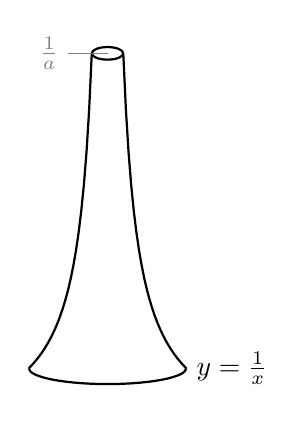
\begin{tikzpicture}
\YEaaxis{2}{2}{1}{5.5}
\draw[thick] plot[domain=.2:1](\x,{1/\x}) node[right]{$y=\frac{1}{x}$};
\draw[thick] plot[domain=.2:1](-\x,{1/\x});
\YExcoord{1}{1}
\YExcoord{0.2}{a\vphantom{1}}
\YExcoord{-1}{-1}
\draw[thick] (-1,1) arc(180:360: 1 cm and 2mm);
\draw[thick] (-.2,5) arc(180:360: .2 cm and .8mm);
\draw[thick] (-.2,5) arc(180:0: .2 cm and .8mm);
\draw[gray] (0,5)--(-.5,5) node[left]{$\frac{1}{a}$};
\end{tikzpicture}
\end{center}
True or false: \textcolor{blue}{No matter how large a constant $M$ is, there is some value of $a$ that makes a solid with volume larger than $M$.}
\end{Mquestion}
\begin{hint}
To find the volume of the solid, cut it into horizontal slices, which are thin circular disks.

The true/false statement is equivalent to saying that the improper integral giving the volume of the solid when $a=0$ diverges to infinity.
\end{hint}
\begin{answer}
false
\end{answer}
\begin{solution}
To find the volume of the solid, we cut it into horizontal slices, which are thin circular disks. At height $y$, the disk has radius $x=\frac{1}{y}$ and thickness $\dee{y}$, so its volume is $\frac{\pi}{y^2}\dee{y}$. The base of the solid is at height $y=1$, and its top is at height $y=\frac{1}{a}$. So, the volume of the entire solid is:
\begin{align*}
\int_1^{1/a} \frac{\pi}{y^2}\dee{y} = \left[-\frac{\pi}{y}\right]_1^{1/a} = \pi (1-a)
\end{align*}
If we imagine sliding $a$ closer and closer to 0, the volume increases, getting closer and closer to $\pi$ units, but never quite reaching it.

So, the statement is false. For example, if we set $M=4$, no matter which $a$ we choose our solid has volume strictly less than $M$.

Remark: we've seen before that $\int_0^1 \frac{1}{x}\,\dee{x}$ diverges. If we imagine the solid that would result from choosing $a=0$, it would have a scant volume of $\pi$ cubic units, but a silhouette (side view) of infinite area.
\end{solution}
%%%%%%%%%%%%%%%%%%%


%%%%%%%%%%%%%%%%%%%

\begin{question}[2016Q4]
What is the largest value of $q$ for which the integral
$\displaystyle \int_1^\infty \frac1{x^{5q}}\,\dee{x}$ diverges?
\end{question}

\begin{hint}
Review Example \eref{CLP101}{eg:IMPp1} in the
%\href{http://www.math.ubc.ca/%7Efeldman/m101/clp/clp_notes_101.pdf}{CLP--II text}.
CLP--II text. Remember the antiderivative of $\frac{1}{x}$ looks very different from the antiderivative of other powers of $x$.
\end{hint}

\begin{answer}
$q=\frac{1}{5}$
\end{answer}

\begin{solution}
Our goal is to decide when this integral diverges, and where it converges. We will leave $q$ as a variable, and antidifferentiate. In order to antidifferentiate without knowing $q$, we'll need different cases.
The integrand is $x^{-5q}$, so when $-5q \neq -1$, we use the power rule (that is, $\int x^n~\dee{x} = \frac{x^{n+1}}{n+1}$) to antidifferentiate.  Note $x^{(-5q)+1} = x^{1-5q} = \dfrac{1}{x^{5q-1}}$.
\begin{align*}
\int_1^t \frac1{x^{5q}}\,\dee{x} &= \begin{cases}
\left[\frac{x^{1-5q}}{1-5q} \right]_1^t \text{ with }1-5q>0 &\text{if } q < \frac15 \\[10pt]
\left[ \log x\vphantom{\frac12}\right]_1^{t}\  &\text{if } q = \frac15 \\[10pt]
\left[\frac{1}{(1-5q)x^{5q-1}} \right]_1^{t}\text{ with }5q-1>0 &\text{if } q > \frac15
\end{cases}\\
&=\begin{cases}
\frac1{1-5q}(t^{1-5q}-1) \text{ with }1-5q>0 &\text{if } q < \frac15 \\
\log t &\text{if } q = \frac15 \\
\frac1{5q-1}(1-\frac1{t^{5q-1}})\text{ with }5q-1>0 &\text{if } q > \frac15.
\end{cases}
\end{align*}
Therefore,
\begin{align*}
\int_1^\infty \frac1{x^{5q}}\,\dee{x} = \displaystyle\lim_{t\to\infty} \left( \int_1^t \frac1{x^{5q}}\,\dee{x} \right) = \begin{cases}
\frac1{1-5q}\left(\displaystyle\lim_{t\to\infty} t^{1-5q}-1\right) = \infty &\text{if } q < \frac15 \\[10pt]
\displaystyle\lim_{t\to\infty}\log t = \infty &\text{if } q = \frac15 \\[10pt]
\frac1{5q-1}\left(1-\displaystyle\lim_{t\to\infty}\frac1{t^{5q-1}}\right) = \frac1{5q-1} &\text{if } q > \frac15.
\end{cases}
\end{align*}
The first two cases are divergent, and so the largest such value is $q=\frac{1}{5}$. (Alternatively, we might recognize this as a ``$p$-integral'' with $p=5q$, and recall that the $p$-integral diverges precisely when $p\le1$.)

\end{solution}

%%%%%%%%%%%%%%%%%%%

\begin{Mquestion}
For which values of $p$ does the integral $\displaystyle\int_0^\infty \dfrac{x}{(x^2+1)^p}~\dee{x}$ converge?
\end{Mquestion}
\begin{hint}
Compare to Example~\eref{CLP101}{eg:IMPp11} in the CLP--II text. You can antidifferentiate with a $u$-substitution.
\end{hint}
\begin{answer}
$p>1$
\end{answer}
\begin{solution}
This integrand is a nice candidate for the substitution $u=x^2+1$, $\frac{1}{2}\dee{u} = x\dee{x}$. Remember when we use substitution on a definite integral, we also need to adjust the limits of integration.
\begin{align*}
\int_0^\infty \dfrac{x}{(x^2+1)^p}~\dee{x} &= \lim_{t \to \infty}\int_0^t \frac{x}{(x^2+1)^p}\dee{x}\\
&=\lim_{t \to \infty}\frac{1}{2}\int_1^{t^2+1} \dfrac{1}{u^p}~\dee{u}\\
&=\lim_{t \to \infty}\frac{1}{2}\int_1^{t^2+1}u^{-p}~\dee{u}\\
&=\begin{cases}
\frac12\displaystyle\lim_{t \to \infty}\left[\frac{u^{1-p}}{1-p}\right]_1^{t^2+1}&\text{ if }p \neq 1\\[7pt]
\frac12\displaystyle\lim_{t \to \infty}\Big[\log|u|\Big]_1^{t^2+1}&\text{ if }p=1
\end{cases}\\
&=\begin{cases}
\frac12\displaystyle\lim_{t \to \infty}\frac{1}{1-p}\left[(t^2+1)^{1-p}-1\right]&\text{ if }p \neq 1\\[7pt]
\frac12\displaystyle\lim_{t \to \infty}\Big[\log(t^2+1)\Big]=\infty&\text{ if }p=1
\end{cases}
\intertext{
At this point, we can see that the integral diverges when $p=1$. When $p \neq 1$, we have the limit }
\displaystyle\lim_{t \to \infty}\frac{1/2}{1-p}\left[(t^2+1)^{1-p}-1\right]&=\frac{1/2}{1-p}\left[\lim_{t \to \infty} (t^2+1)^{1-p}\right] - \frac{1/2}{1-p}
\end{align*}
Since $t^2+1 \to \infty$, this limit converges exactly when the exponent $1-p$ is negative; that is, it converges when $p>1$, and diverges when $p<1$.

So, the integral in the question converges when $p>1$.
\end{solution}

%%%%%%%%%%%%%%%%%%%
\begin{question}
Evaluate $\displaystyle\int_2^\infty  \frac{1}{t^4-1}\dee{t}$, or state that it diverges.
\end{question}
\begin{hint}
To evaluate the integral, you can factor the denominator. \\
Recall $\displaystyle\lim_{x \to \infty}\arctan x = \frac{\pi}{2}$. For the other limits, use logarithm rules, and beware of indeterminate forms.
\end{hint}
\begin{answer}
$\dfrac{\log 3-\pi}{4} + \dfrac{1}{2}\arctan 2 $
\end{answer}
\begin{solution}
\begin{itemize}
\item First, we notice there is only one ``source of impropriety:"  the domain of integration is infinite.  (The integrand has a singularity at $t=1$, but this is not in the domain of integration, so it's not a problem for us.)
\item We should try to get some intuition about whether the integral converges or diverges.  When $t \to \infty$, notice the integrand ``looks like" the function $\frac{1}{t^4}$. We know $\int_1^\infty \frac{1}{t^4}~\dee{t}$ converges, because it's a $p$-integral with $p=4>1$ (see Example~\eref{CLP101}{eg:IMPp1} in the CLP--II text). So, our integral probably converges as well. If we were only asked show it converges, we could use a comparison test, but we're asked more than that.
\item Since we guess the integral converges, we'll need to evaluate it. The integrand is a rational function, and there's no obvious substitution, so we use partial fractions.
\end{itemize}
\begin{align*}
\frac{1}{t^4-1} &= \frac{1}{(t^2+1)(t^2-1)}= \frac{1}{(t^2+1)(t+1)(t-1)} = \frac{At+B}{t^2+1} + \frac{C}{t+1}+\frac{D}{t-1}
\intertext{Multiply by the original denominator.}
1&=(At+B)(t+1)(t-1) + C(t^2+1)(t-1) +D(t^2+1)(t+1)\tag{$*$}
\intertext{Set $t=1$.}
1&=0+0+D(2)(2) \qquad \Rightarrow \qquad \color{red}D=\frac{1}{4}
\intertext{Set $t=-1$.}
1&=0+C(2)(-2)+0 \qquad \Rightarrow \qquad \color{red}C=-\frac{1}{4}
\intertext{Simplify ($*$) using $D=\frac{1}{4}$ and $C=-\frac{1}{4}$.}
1&=(At+B)(t+1)(t-1) \textcolor{red}{-\frac{1}{4}}(t^2+1)(t-1) +\textcolor{red}{\frac{1}{4}}(t^2+1)(t+1)\\
&=(At+B)(t+1)(t-1) + \frac{1}{2}(t^2+1)\\
&=At^3+\left(B+\frac{1}{2}\right)t^2-At+\left(\frac{1}{2}-B\right)
\intertext{By matching up coefficients of corresponding powers of $t$, we find \textcolor{red}{$A=0$} and \textcolor{red}{$B=-\frac{1}{2}$}.}
\int_2^\infty \frac{1}{t^4-1}~\dee{t}&=\int_2^\infty \left( \frac{-1/2}{t^2+1}  - \frac{1/4}{t+1}+\frac{1/4}{t-1}\right)~\dee{t}\\
&=\lim_{R \to \infty}\int_2^R \left( \frac{-1/2}{t^2+1}  - \frac{1/4}{t+1}+\frac{1/4}{t-1}\right)~\dee{t}\\
&=\lim_{R \to \infty} \left[-\frac{1}{2}\arctan t - \frac{1}{4}\log|t+1|+\frac{1}{4}\log|{t-1}|\right]_2^R\\
&=\lim_{R \to \infty} \left[-\frac{1}{2}\arctan t + \frac{1}{4}\log\left| \frac{t-1}{t+1} \right|\right]_2^R\\
&=\lim_{R \to \infty} \left(-\frac{1}{2}\arctan R +\frac12\arctan 2 + \frac{1}{4}\log\left| \frac{R-1}{R+1} \right|-\frac{1}{4}\log\left| \frac{2-1}{2+1} \right|\right)
\intertext{We can use l'H\^opital's rule to see $\displaystyle\lim_{R \to \infty}\frac{R-1}{R+1}=1$. Also note $-\log (1/3) = \log 3$.}
&=-\frac{1}{2}\left(\frac{\pi}{2}\right) +\frac{1}{2}\arctan 2 + \frac{1}{4}\log1+\frac{1}{4}\log3\\
&=\frac{\log 3-\pi}{4} + \frac{1}{2}\arctan 2
\end{align*}
\end{solution}

%%%%%%%%%%%%%%%%%%%
\begin{question}
Does the integral $\displaystyle\int_{-5}^5 \left(\frac{1}{\sqrt{|x|}} + \frac{1}{\sqrt{|x-1|}}+\frac{1}{\sqrt{|x-2|}}\right)\dee{x}$ converge or diverge?
\end{question}
\begin{hint}
Break up the integral. The absolute values give you a nice even function, so you can replace $|x-a|$ with $x-a$ if you're careful about the limits of integration.
\end{hint}
\begin{answer}
The integral converges.
\end{answer}
\begin{solution}
There are three singularities in the integrand: $x=0$, $x=1$, and $x=2$. We'll need to break up the integral at each of these places.
\begin{align*}
&\int_{-5}^5 \left(\frac{1}{\sqrt{|x|}} + \frac{1}{\sqrt{|x-1|}}+\frac{1}{\sqrt{|x-2|}}\right)\dee{x}\\
=
&\int_{-5}^0 \left(\frac{1}{\sqrt{|x|}} + \frac{1}{\sqrt{|x-1|}}+\frac{1}{\sqrt{|x-2|}}\right)\dee{x}+
\int_{0}^1 \left(\frac{1}{\sqrt{|x|}} + \frac{1}{\sqrt{|x-1|}}+\frac{1}{\sqrt{|x-2|}}\right)\dee{x}\\+&
\int_{1}^2 \left(\frac{1}{\sqrt{|x|}} + \frac{1}{\sqrt{|x-1|}}+\frac{1}{\sqrt{|x-2|}}\right)\dee{x}+
\int_{2}^5 \left(\frac{1}{\sqrt{|x|}} + \frac{1}{\sqrt{|x-1|}}+\frac{1}{\sqrt{|x-2|}}\right)\dee{x}
\end{align*}
This looks rather unfortunate. Let's think again. If all of the integrals below converge, then we can write:
\begin{align*}
\int_{-5}^5 \left(\frac{1}{\sqrt{|x|}} + \frac{1}{\sqrt{|x-1|}}+\frac{1}{\sqrt{|x-2|}}\right)\dee{x}&=
\int_{-5}^5 \frac{1}{\sqrt{|x|}} \dee{x}+
\int_{-5}^5 \frac{1}{\sqrt{|x-1|}}\dee{x}+
\int_{-5}^5\frac{1}{\sqrt{|x-2|}}\dee{x}
\intertext{That looks a lot better. Also, we have a good reason to guess these integrals converge--they look like $p$-integrals with $p=\frac{1}{2}$. Let's take a closer look at each one.}
\int_{-5}^5 \frac{1}{\sqrt {|x|}}\dee{x}&=\int_{-5}^0 \frac{1}{\sqrt {|x|}}\dee{x}+
\int_{0}^5 \frac{1}{\sqrt {|x|}}\dee{x}\\
&=2\int_{0}^5 \frac{1}{\sqrt {|x|}}\dee{x} \qquad\text{(even function)}\\
&=2\int_{0}^5 \frac{1}{\sqrt {x}}\dee{x}
\intertext{This is a $p$-integral, with $p=\frac{1}{2}$. By Example~\eref{CLP101}{eg:IMPp2}
 in the CLP--II text (and Theorem~\eref{CLP101}{thm:IMPfiniteSHift}, since the upper limit of integration is not 1), it converges. The other two pieces behave similarly.}
\int_{-5}^5 \frac{1}{\sqrt{|x-1|}}\dee{x}&=
\int_{-5}^1 \frac{1}{\sqrt{|x-1|}}\dee{x}+
\int_{1}^5 \frac{1}{\sqrt{|x-1|}}\dee{x}
\intertext{Use $u=x-1$, $\dee{u}=\dee{x}$}
&=
\int_{-6}^0 \frac{1}{\sqrt{|u|}}\dee{u}+
\int_{0}^4 \frac{1}{\sqrt{|u|}}\dee{x}
\\&=
\int_{0}^6 \frac{1}{\sqrt{u}}\dee{u}+
\int_{0}^4 \frac{1}{\sqrt{u}}\dee{x}
\intertext{Since our function is even, we use the reasoning of Example~\eref{CLP101}{eg:lefthalfevenfunction} in the CLP--II text to consider the area under the curve when $x \ge 0$, rather than when $x\leq 0$. Again, these are $p$-integrals with $p = \frac{1}{2}$, so they both converge. Finally:}
\int_{-5}^5\frac{1}{\sqrt{|x-2|}}\dee{x}&=
\int_{-5}^2\frac{1}{\sqrt{|x-2|}}\dee{x}+
\int_{2}^5\frac{1}{\sqrt{|x-2|}}\dee{x}
\intertext{Use $u=x-2$, $\dee{u}=\dee{x}$.}
&=
\int_{-7}^0\frac{1}{\sqrt{|u|}}\dee{u}+
\int_{0}^3\frac{1}{\sqrt{|u|}}\dee{u}\\
&=
\int_{0}^7\frac{1}{\sqrt{u}}\dee{u}+
\int_{0}^3\frac{1}{\sqrt{u}}\dee{u}
\intertext{Since $p = \frac{1}{2}$, so they both converge.}
\end{align*}
We conclude our original integral, as the sum of convergent integrals, converges.
\end{solution}



%%%%%%%%%%%%%%%%%%%
\begin{Mquestion}
Evaluate $\displaystyle\int_0^\infty e^{-x}\sin x~\dee{x}$, or state that it diverges.
\end{Mquestion}
\begin{hint}
Use integration by parts twice to find the antiderivative of $e^{-x}\sin x$, as in Example~\eref{CLP101}{eg:circularint} of the CLP--II text. Be careful with your signs ---
it's easy to make a mistake with all those negatives.

If you're having a hard time taking the limit at the end, review the Squeeze Theorem, Theorem~\eref{CLP100}{thm squeeze} in the CLP--I text.
\end{hint}
\begin{answer}
$\dfrac{1}{2}$
\end{answer}
\begin{solution}
We can use integration by parts twice to find the antiderivative of $e^{-x}\sin x$, as in Example~\eref{CLP101}{eg:circularint} of the CLP--II text. To keep our work a little simpler, we'll find the antiderivative first, then take the limit.

Let $u=e^{-x}$, $\dee{v}=\sin x~\dee{x}$, so $\dee{u}=-e^{-x}~\dee{x}$ and $v=-\cos x$.
\begin{align*}
\int e^{-x}\sin x~\dee{x}&=-e^{-x}\cos x - \int e^{-x}\cos x~\dee{x}
\intertext{Now let $u=e^{-x}$, $\dee{v}=\cos x~\dee{x}$, so $\dee{u}=-e^{-x}~\dee{x}$ and $v=\sin x$.}
&=-e^{-x}\cos x-\left[e^{-x}\sin x + \int e^{-x}\sin x~\dee{x} \right]\\
&=-e^{-x}\cos x-e^{-x}\sin x - \int e^{-x}\sin x~\dee{x}
\intertext{All together, we found}
\color{red}\int e^{-x}\sin x~\dee{x}&=-e^{-x}\cos x-e^{-x}\sin x -\color{red} \int e^{-x}\sin x~\dee{x} \color{black}+C\\
\color{red}2\int e^{-x}\sin x~\dee{x}&=-e^{-x}\cos x-e^{-x}\sin x +C\\
\int e^{-x}\sin x~\dee{x}&=-\frac{1}{2e^x}(\cos x+\sin x) +C
\intertext{(Remember, since $C$ is an arbitrary constant, we can rename $\frac{C}{2}$ to simply $C$.) Now we can evaluate our improper integral.}
\int_0^\infty e^{-x}\sin x~\dee{x}&=
\lim_{b \to \infty}\int_0^b e^{-x}\sin x~\dee{x}\\
&=
\lim_{b \to \infty}\left[-\frac{1}{2e^x}(\cos x+\sin x) \right]_0^b
\\&=
\lim_{b \to \infty}\left(\frac{1}{2}-\frac{1}{2e^b}(\cos b+\sin b) \right)
\intertext{To find the limit, we use the Squeeze Theorem (Theorem~\eref{CLP100}{thm squeeze} in the CLP--I text). Since $|\sin b|,|\cos b| \leq 1$ for any $b$, we can use the fact that $-2 \le \cos b + \sin x \le 2$ for any $b$.}
&\qquad\frac{-2}{2e^b} \leq \frac{1}{2e^b}(\cos b + \sin b)  \leq \frac{2}{2e^b}\\
&\qquad\lim_{b \to \infty}\frac{-2}{2e^b} = 0 = \frac{2}{2e^b}\\
&\qquad\mbox{So, }\qquad\lim_{b \to \infty}\left[\frac{1}{2e^b}(\cos b + \sin b)\right]=0\\
\mbox{Therefore, }\qquad\frac{1}{2}&=
\lim_{b \to \infty}\left(\frac{1}{2}-\frac{1}{2e^b}(\cos b+\sin b) \right)
\end{align*}
That is, $\displaystyle\int_0^\infty e^{-x}\sin x~\dee{x}= \frac{1}{2}$.
\end{solution}

%%%%%%%%%%%%%%%%%%

\begin{question}[M121 2002A]
Is the integral $\displaystyle\int_0^\infty\frac{\sin^4 x}{x^2}\, \dee{x}$
convergent or divergent? Explain why.
\end{question}

\begin{hint}
What is the limit of the integrand when $x\rightarrow 0$?
\end{hint}

\begin{answer}
The integral converges.
\end{answer}

\begin{solution}
The integrand is positive everywhere. So either the integral
converges to some finite number or it is infinite. There are two potential
``sources of impropriety'' --- a possible singularity at $x=0$ and
the fact that the domain of integration extends to $\infty$.
So, we split up the integral.
\begin{equation*}
\int_0^\infty\frac{\sin^4 x}{x^2}\, \dee{x}
=\int_0^1\frac{\sin^4 x}{x^2}\, \dee{x}
  + \int_1^\infty\frac{\sin^4 x}{x^2}\, \dee{x}
\end{equation*}

Let's consider the first integral. By l'H\^opital's rule
(or recall Example \eref{CLP100}{eg:hopitalA} in the CLP--I text),
\begin{equation*}
\lim_{x\to 0} \frac{\sin x}{x}
=\lim_{x\to 0} \frac{\cos x}{1}
=\cos 0
=1
\end{equation*}
Consequently,
\begin{equation*}
\lim_{x\to 0} \frac{\sin^4 x}{x^2}
=\Big(\lim_{x\to 0} \sin^2 x \Big)
\Big(\lim_{x\to 0} \frac{\sin x}{x} \Big)
\Big(\lim_{x\to 0} \frac{\sin x}{x} \Big)
=0\times 1\times 1
=0
\end{equation*}
and the first integral is not even improper.

Now for the second integral. Since $|\sin x|\le 1$, we'll compare it to $\int_1^\infty \frac{1}{x^2}$.
\begin{itemize}
\item $\frac{\sin^4 x}{x^2}$ and $\frac{1}{x^2}$ are defined and continuous for every $x \geq 1$
\item $0 \leq \frac{\sin^4 x}{x^2} \leq \frac{1^4}{x^2} = \frac{1}{x^2}$ for every $x \geq 1$
\item $\int_1^\infty \frac{1}{x^2}~\dee{x}$ converges by Example~\eref{CLP101}{eg:IMPp1}
 in the CLP--II text (it's a $p$-type integral with $p>1$)
\end{itemize}

By the comparison test, Theorem~\eref{CLP101}{thm:IMPcomparison} in the CLP--II text,
$\displaystyle\int_1^\infty\frac{\sin^4 x}{x^2}\, \dee{x}$ converges.

Since $\displaystyle\int_0^1\frac{\sin^4 x}{x^2}\, \dee{x}$ and $\displaystyle\int_1^\infty\frac{\sin^4 x}{x^2}\, \dee{x}$ both converge, we conclude
$\displaystyle\int_0^\infty\frac{\sin^4 x}{x^2}\, \dee{x}$ converges as well.
\end{solution}


%%%%%%%%%%%%%%%%%%%
\begin{Mquestion}
Does the integral $\displaystyle\int_0^\infty \frac{x}{e^x+\sqrt{x}} ~\dee{x}$ converge or diverge?
\end{Mquestion}
\begin{hint}
The only ``source of impropriety" is the infinite domain of integration.
Don't be afraid to be a little creative to make a comparison work.
\end{hint}
\begin{answer}
The integral converges.
\end{answer}
\begin{solution}
Since the denominator is positive for all $x \geq 0$, the integrand is continuous over $[0, \infty)$. So, the only ``source of impropriety" is the infinite domain of integration.

\begin{description}
\item[Solution 1:] Let's try to use a direct comparison. Note $\dfrac{x}{e^x + \sqrt{x}} \geq 0$ whenever $x \geq 0$. Also note that, for large values of $x$, $e^x$ is much larger than $\sqrt{x}$. That leads us to consider the following inequalty:
\[
0\leq \dfrac{x}{e^x + \sqrt{x}}  \leq \dfrac{x}{e^x }\]

If $\int_0^\infty \frac{x}{e^x}~\dee{x}$ converges, we're in business. Let's figure it out. The integrand looks like a candidate for integration by parts: take $u=x$, $\dee{v} = e^{-x}~\dee{x}$, so $\dee{u}=\dee{x}$ and $v=-e^{-x}$.
\begin{align*}
\int_0^\infty \frac{x}{e^x}~\dee{x}&=\lim_{b \to \infty}\int_0^b \frac{x}{e^x}~\dee{x}=
\lim_{b \to \infty}\left( \left[-\frac{x}{e^x}\right]_0^b + \int_0^b e^{-x}~\dee{x} \right)\\&=
\lim_{b \to \infty}\left(-\frac{b}{e^b} +\left[-e^{-x}\right]_0^b \right)=
\lim_{b \to \infty}\left(-\frac{b}{e^b} -\frac{1}{e^b}+1 \right)\\&=
\lim_{b \to \infty}\bigg(1-\underbrace{\frac{b+1}{e^b}}_{\atp{\mathrm{num}\to\infty}{\mathrm{den}\to\infty}}  \bigg)=\lim_{b \to \infty}\bigg(1-\frac{1}{e^b} \bigg)=1
\end{align*}
Using l'H\^{o}pital's rule, we see $\int_0^\infty \frac{x}{e^x}~\dee{x}$ converges.  All together:
\begin{itemize}
\item $\frac{x}{e^x}$ and $\frac{x}{e^x+\sqrt{x}}$ are defined and continuous for all $x \geq 0$,
\item $\left|\frac{x}{e^x+\sqrt{x}}\right|\leq \frac{x}{e^x}$, and
\item $\int_0^\infty \frac{x}{e^x}~\dee{x}$ converges.
\end{itemize}
So, by Theorem~\eref{CLP101}{thm:IMPcomparison} in the CLP--II text, our integral $\displaystyle\int_0^\infty \frac{x}{e^x+\sqrt{x}} ~\dee{x}$ converges.

\item[Solution 2:]
Let's try to use a different direct comparison from Solution 1, and avoid integration by parts.
We'd like to compare to something like $\dfrac{1}{e^x}$, but the inequality goes the wrong way. So, we make a slight modification: we consider $2e^{-x/2}$. To that end, we claim $x<2e^{x/2}$ for all $x \geq 0$. We can prove this by noting the following two facts:
\begin{itemize}
\item $0<2=2e^{0/2}$, and
\item  $\diff{}{x}\{x\} = 1 \le e^{x/2} = \diff{}{x}\{2e^{x/2}\}$. \end{itemize}
So, when $x=0$, $x < 2e^{x/2}$, and then as $x$ increases, $2e^{x/2}$ grows faster than $x$.

Now we can make the following comparison:
\begin{align*}
0\leq \dfrac{x}{e^x + \sqrt{x}}  &\leq \dfrac{x}{e^x } <\frac{2e^{x/2}}{e^x} = \frac{2}{e^{x/2}}
\intertext{We have a hunch that $\int_0^\infty \frac{2}{e^{x/2}}~\dee{x}$ converges, just like $\int_0^\infty \frac{1}{e^{x}}~\dee{x}$. This is easy enough to prove. We can guess an antiderivative, or use the substitution $u=x/2$.}
\int_0^\infty \frac{2}{e^{x/2}}~\dee{x}&=\lim_{R \to \infty} \int_0^R \frac{2}{e^{x/2}}~\dee{x} =\lim_{R \to \infty} \left[- \frac{4}{e^{x/2}}\right]_0^R\\
&=\lim_{R \to \infty} \left[\frac{4}{e^{0}}- \frac{4}{e^{R/2}}\right]_0^R=4
\end{align*}
Now we know:
\begin{itemize}
\item $0 \leq \frac{x}{e^x+\sqrt{x}} \leq \frac{2}{e^{x/2}}$, and
\item $\int_0^\infty \frac{2}{e^{x/2}}~\dee{x}$ converges.
\item Furthermore,  $\frac{x}{e^x+\sqrt{x}}$ and $\frac{2}{e^{x/2}}$ are defined and continuous for all $x \geq 0$.
\end{itemize}
By the comparison test (Theorem~\eref{CLP101}{thm:IMPcomparison}) in the CLP--II text,
we conclude the integral converges.

\item[Solution 3:] Let's use the limiting comparison test (Theorem~\eref{CLP101}{thm:IMPcomparisonLim} in the CLP--II text).
We have a hunch that our integral behaves similarly to $\int_0^\infty \frac{1}{e^x}\,\dee{x}$, which converges (see Example~\eref{CLP101}{eg:IMPp6} in the CLP--II text). Unfortunately, if we choose $g(x) = \frac{1}{e^x}$ (and, of course, $f(x) = \frac{x}{e^x+\sqrt{x}}$), then
\[\lim_{x \to \infty}\frac{f(x)}{g(x)} =
\lim_{x \to \infty}\frac{x}{e^x+\sqrt{x}}\cdot e^x =
\lim_{x \to \infty}\frac{x}{1+\underbrace{\tfrac{\sqrt{x}}{e^x}}_{\to 0}} = \infty\]
That is, the limit does not exist, so the limiting comparison test does not apply. (To find $\lim\limits_{x \to \infty}\frac{\sqrt{x}}{e^x}$, you can use l'H\^{o}pital's rule.)

This setback encourages us to try a slightly different angle. If $g(x)$ gave larger values, then we could decrease $\frac{f(x)}{g(x)}$. So, let's try $g(x) = \frac{1}{e^{x/2}} = e^{-x/2}$. Now,
\begin{align*}
\lim_{x \to \infty}\frac{f(x)}{g(x)} &=
\lim_{x \to \infty}\frac{x}{e^x+\sqrt{x}}\div \frac{1}{e^{x/2}}=
\lim_{x \to \infty}\frac{x}{e^{x/2}+\frac{\sqrt{x}}{e^{x/2}}}
\end{align*}
Hmm... this looks hard. Instead of dealing with it directly, let's use the squeeze theorem, Theorem~\eref{CLP100}{thm squeeze} in the CLP--I text.
\begin{align*}
0 &&\leq&& \frac{x}{e^{x/2}+\frac{\sqrt{x}}{e^{x/2 }}}&&\leq&& \frac{x}{e^{x/2}}
\end{align*}
Using l'H\^{o}pital's rule,
\[\lim_{x \to \infty} \underbrace{\frac{x}{e^{x/2}}}_{\atp{\mathrm{num}\to \infty}{\mathrm{den}\to\infty}} = \lim_{x \to \infty}\frac{1}{\frac{1}{2}e^{x/2}}=0 = \lim_{x \to \infty}0\]
So, by the squeeze theorem $\lim\limits_{x \to 0}\frac{\frac{x}{e^x+\sqrt{x}}}{\frac{1}{e^{x/2}}}=0$. Since this limit exists, $\frac{1}{e^{x/2}}$ is a reasonable function to use in the limiting comparison test (provided its integral converges). So, we need to show that $\int_0^\infty \frac{1}{e^{x/2}}\,\dee{x}$ converges. This can be done by simply evaluating it:

\[\int_0^\infty \frac{1}{e^{x/2}}\,\dee{x} = \lim_{b \to \infty}\int_0^b {e^{-x/2}}\,\dee{x}
= \lim_{b \to \infty} -\frac{1}{2}\big[e^{-x/2}\big]_0^b
= \lim_{b \to \infty} -\frac{1}{2}\left[\frac{1}{e^{b/2}}-1\right] = \frac{1}{2}\]

So, all together:

\begin{itemize}
\item The functions $\frac{x}{e^x+\sqrt{x}}$ and $\frac{1}{e^{x/2}}$ are defined and continuous for all $x \geq 0$, and $\frac{1}{e^{x/2}} \ge 0$ for all $x \ge 0$.
\item $\int_0^\infty \frac{1}{e^{x/2}}\,\dee{x}$ converges.
\item The limit $\lim\limits_{x \to \infty}\frac{\frac{x}{e^x}+\sqrt{x}}{\frac{1}{e^{x/2}}}$ exists (it's equal to 0).
\item So, the limiting comparison test (Theorem~\eref{CLP101}{thm:IMPcomparison}
in the CLP--II text) tells us that $\int_0^\infty \frac{x}{e^x+\sqrt{x}}\,\dee{x}$ converges as well.
\end{itemize}
\end{description}

\end{solution}

%%%%%%%%%%%%%%%%%%%

\begin{question}[M121 2001A]
Let $M_{n,t}$ be the Midpoint Rule approximation for
$\displaystyle\int_0^t \frac{e^{-x}}{1+x}\ \dee{x}$ with $n$ equal subintervals.
Find a value of $t$ and a value of $n$ such that $M_{n,t}$ differs
from  $\int_0^\infty \frac{e^{-x}}{1+x}\ \dee{x}$ by at most $10^{-4}$.
Recall that the error $E_n$ introduced when the Midpoint
Rule is used with $n$ subintervals obeys
\begin{align*}
|E_n|\le \frac{M(b-a)^3}{24n^2}
\end{align*}
where $M$ is the maximum absolute value of the second derivative of the
integrand and $a$ and $b$ are the end points of the interval of integration.
\end{question}

\begin{hint}
There are two things that contribute to your error: using $t$ as the upper bound instead of infinity, and using $n$ intervals for the approximation.

First, find a $t$ so that the error introduced by approximating
$\int_0^\infty \frac{e^{-x}}{1+x}\ \dee{x}$ by $\int_0^t \frac{e^{-x}}{1+x}\ \dee{x}$
is at most $\frac{1}{2} 10^{-4}$. Then, find your $n$.
\end{hint}

\begin{answer}
$t=10$ and $n= 2042$ will do the job.
There are many other correct answers.
\end{answer}

\begin{solution}
There are two sources of error: the upper bound is $t$, rather than infinity, and we're using an approximation with some finite number of intervals, $n$. Our plan is to first find a value of $t$ that introduces an error of no more than $\frac{1}{2}10^{-4}$. That is, we'll find a value of $t$ such that $\int_t^\infty \frac{e^{-x}}{1+x}~\dee{x} \leq \frac{1}{2}10^{-4}$. After that, we'll find a value of $n$ that approximates $\int_0^t \frac{e^{-x}}{x+1}~\dee{x}$ to within $\frac{1}{2}10^{-4}$. Then, all together, our  error will be at most $\frac{1}{2}10^{-4} + \frac{1}{2}10^{-4} = 10^{-4}$, as desired. (Note we could have broken up the error in another way---it didn't have to be $\frac{1}{2}10^{-4}$ and $\frac{1}{2}10^{-4}$. This will give us one of many possible answers.)

Let's  find a $t$ such that
$\int_t^\infty  \frac{e^{-x}}{1+x}\ \dee{x}\le\frac{1}{2} 10^{-4}$.
For all $x\ge 0$,
$0<\frac{e^{-x}}{1+x}\le e^{-x}$, so
\begin{align*}
\int_t^\infty  \frac{e^{-x}}{1+x}\ \dee{x}
\le \int_t^\infty e^{-x}\ \dee{x}
=e^{-t}&\stackrel{(*)}{\le}\frac{1}{2} 10^{-4}\\
\hbox{where ($*$) is true if }\quad
t&\ge -\log\Big(\frac{1}{2} 10^{-4}\Big)\approx 9.90
\end{align*}
Choose, for example, $t=10$.

Now it's time to decide how many intervals we're going to use to approximate $\displaystyle\int_0^t \frac{e^{-x}}{x+1}~\dee{x}$. Again, we want our error to be less than $\frac{1}{2}10^{-4}$. To bound our error, we need to know the second derivative of $\frac{e^{-x}}{x+1}$.
\begin{align*}
f(x)=\frac{e^{-x}}{1+x}
\implies f'(x)=-\frac{e^{-x}}{1+x}-\frac{e^{-x}}{(1+x)^2}
\implies f''(x)&=\frac{e^{-x}}{1+x}+2\frac{e^{-x}}{(1+x)^2}
+2\frac{e^{-x}}{(1+x)^3}
\end{align*}
Since $f''(x)$ is positive, and decreases as $x$ increases,
\begin{align*}
|f''(x)|\le f''(0) = 5
\implies |E_n|\le\frac{5(10-0)^3}{24n^2}=\frac{5000}{24n^2}
=\frac{625}{3n^2}
\end{align*}
and $|E_n|\le \frac{1}{2} 10^{-4}$ if
\begin{alignat*}{3}
&&\frac{625}{3n^2}&\le \frac{1}{2} 10^{-4}\\
&\iff\qquad &
n^2&\ge \frac{1250\times 10^4}{3}\\
&\iff\quad &n&\ge \sqrt{\frac{1.25\times 10^7}{3}}
\approx 2041.2
\end{alignat*}
So $t=10$ and $n= 2042$ will do the job.
There are many other correct answers.
\end{solution}
%%%%%%%%%%%%%%%%%%%
%%%%%%%%%%%%%%%%%%%


\begin{Mquestion}
Suppose $f(x)$ is continuous for all real numbers, and $\displaystyle\int_1^\infty f(x)~\dee{x}$ converges.
\begin{enumerate}[(a)]
\item If $f(x)$ is odd, does $\displaystyle\int_{-\infty\vphantom{\frac12}}^{-1} f(x)~\dee{x}$ converge or diverge, or is there not enough information to decide?
\item If $f(x)$ is even, does $\displaystyle\int_{-\infty}^\infty f(x)~\dee{x}$ converge or diverge, or is there not enough information to decide?
\end{enumerate}
\end{Mquestion}
\begin{hint}
Look for a place to use Theorem~\eref{CLP101}{thm:IMPfiniteSHift} of the CLP--II text.

 Examples~\eref{CLP101}{eg:lefthalfevenfunction} and \eref{CLP101}{eg:areaunderoddfunction}
 in the CLP--II text have nice results about the area under an even/odd curve.
\end{hint}
\begin{answer}
(a) The integral converges. \qquad (b) The interval converges.
\end{answer}
\begin{solution}
\begin{enumerate}[(a)]
\item Since $f(x)$ is odd, using the reasoning of Example~\eref{CLP101}{eg:areaunderoddfunction} in the CLP--II text,
\begin{align*}
\int_{-\infty}^{-1} f(x)~\dee{x}&=\lim_{t \to \infty}\int_{-t}^{-1}f(x)~\dee{x}=\lim_{t \to \infty}-\int_{1}^{t} f(x)~\dee{x}=-\lim_{t \to \infty} \int_{1}^{t} f(x)~\dee{x}
\end{align*}
Since $\displaystyle\int_1^\infty f(x)~\dee{x}$ converges, the last limit above converges. Therefore, $\displaystyle\int_{-\infty\vphantom{\frac12}}^{-1} f(x)~\dee{x}$ converges.
\item Since $f(x)$ is even, using the reasoning of Example~\eref{CLP101}{eg:lefthalfevenfunction} in the CLP--II text,
\begin{align*}
\int_{-\infty}^{-1} f(x)~\dee{x}&=\lim_{t \to \infty}\int_{-t}^{-1}f(x)~\dee{x}=\lim_{t \to \infty}\int_{1}^{t} f(x)~\dee{x}=\lim_{t \to \infty} \int_{1}^{t} f(x)~\dee{x}
\intertext{Since $\displaystyle\int_1^\infty f(x)~\dee{x}$ converges, the last limit above converges.  Since $f(x)$ is continuous everywhere, by Theorem~\eref{CLP101}{thm:IMPfiniteSHift}
in the CLP--II text,  $\displaystyle\int_{-1}^\infty f(x)~\dee{x}$ converges (note the adjusted lower limit). Then, since}
\int_{-\infty}^\infty f(x)~\dee{x}& =
\int_{-\infty}^{-1} f(x)~\dee{x} +
\int_{-1}^\infty f(x)~\dee{x}
\end{align*}
and both summands converge, our original integral converges as well.
\end{enumerate}
\end{solution}



%%%%%%%%%%%%%%%%%%%



\begin{question}
True or false:
\textcolor{blue}{There is some real number $x$, with $x \geq 1$, such that $\displaystyle\int_0^x \frac{1}{e^t}~\dee{t} = 1$. }
\end{question}
\begin{hint}
$x$ should be a real number
\end{hint}
\begin{answer}
false
\end{answer}
\begin{solution}
Define $F(x)=
\int_0^x \frac{1}{e^{t}}\dee{t}$.
\begin{align*}
F(x)=\int_0^x \frac{1}{e^{t}}\dee{t}&=\left[-\frac{1}{e^{t}}\right]_0^x
 = \frac{1}{e^0}-\frac{1}{e^{x}}<\frac{1}{e^0}=1
\end{align*}
So, the statement is false: there is no $x$ such that $F(x)=1$. For every real $x$, $F(x) < \frac{1}{e^0}=1$.

We note here that $\displaystyle\lim_{x \to \infty} \int_0^x\frac{1}{e^{t}}\dee{t}=1$. So, as $x$ grows larger, the gap between $F(x)$ and 1 grows infintesimally small. But there is no real value of $x$ where $F(x)$ is exactly equal to 1.

\end{solution}

%%%%%%%%%%%%%%%%%%%
